\documentclass[a4paper]{article}
% Kodowanie latain 2
%\usepackage[latin2]{inputenc}
\usepackage[T1]{fontenc}
% Można też użyć UTF-8
\usepackage[utf8]{inputenc}
\usepackage{listings}
% Język
\usepackage[polish]{babel}
% \usepackage[english]{babel}
\usepackage{graphicx}
% Rózne przydatne paczki:
% - znaczki matematyczne
\usepackage{amsmath, amsfonts}
% - wcięcie na początku pierwszego akapitu
\usepackage{indentfirst}
% - komenda \url w wersji nie tworzącej dodatkowej ramki
\usepackage[pdfborder={0 0 0 0}]{hyperref}
% - dołączanie obrazków
\usepackage{graphics}
% - szersza strona
\usepackage[nofoot,hdivide={2cm,*,2cm},vdivide={2cm,*,2cm}]{geometry}
\usepackage{lmodern}
\usepackage{hyperref}
\frenchspacing
% - brak numerów stron
\pagestyle{empty}

% dane autora
\author{Julia Majkowska}
\title{Dokumentacja projektu}
\date{\today}

% początek dokumentu
\begin{document}
 \maketitle
 
 \section{Krótki opis}
 Program umożliwiający zamianę mapy wysokości na kolorową mapę hipsometryczną. \\
 Będzie umożliwiał:
 \begin{enumerate}

 
 \item{} wybór w nowym okienku pliku źródłowego tablicy wysokosci(obslugiwane będą formaty DTED (Level 0, 1, 2), SRTM (pliki binarne HGT, TIFF, PNG))
 
 \item{} stworzenie własnego zestawu poziomic i odpowiadającej mu palety, przez dodawanie i usuwanie poziomic i przypisywanie im wartosci w metrach oraz koloru 
 
 \item{} zapis poziomic i palety do istniejącego lub nowego pliku,wybranego lub wpisanego w odpowiednim okienku 
 
 \item{} wczytanie zestawu poziomic i palety, zastępując stworzone w oknie poziomice, z pliku wybranego w nowym okienku
 
 \item{} wczytanie poziomic dodając je do palety w okienku, z pliku wybranego w nowym okienku
 
 \item{} skorzystanie z domyślnej palety kolorów
 
 \item{} podgląd mapy dla aktualnej palety i poziomic w nowym oknie po kliknięciu odpowiedniego przycisku 
 
 \item{} zapis nowej mapy do pliku png

  
 \end{enumerate}
 \section{Wymagane biblioteki}
 \begin{enumerate}
\item{Gtk 3.0}
\item{GDK-PixBuf 2.0}
\item{Gdal 1.9}
 \end{enumerate}
 
 
 \section{Kompilacja}
\begin{enumerate}
\item{Linux}

Zainstalować bibilioteki można następującymi komendami\\
sudo apt-get install gdal-bin\\
sudo apt-get install libgtk-3-dev\\
sudo apt-get install build-essential libgdal-dev\\
sudo apt-get install libgtk-3-dev

Aby skompilować można dodać do folderu z plikami programu plik Makefile.\\ 
Następnie wejść z konsoli do folderu zawierającego pliki programu i wpisać komendę 'make'.

Przykładowy Makefile
\begin{lstlisting}
compile = cc `pkg-config --cflags gtk+-3.0 gdal`

all: interfejs.o paleta.o obrazek.o
	$(compile) interfejs.o paleta.o obrazek.o -o caly_program `pkg-config --libs gtk+-3.0 gdal`

interfejs.o: interfejs.c paletalib.h mapa.h
	$(compile) interfejs.c -c -o interfejs.o 

paleta.o: paleta.c paletalib.h
	$(compile) paleta.c -c -o paleta.o 
	
obrazek.o: obrazek.c paletalib.h mapa.h
	$(compile) obrazek.c -c -o obrazek.o

\end{lstlisting}



\item{Windows}

Można stworzyć projekt w CodeBlocksie dopisując w opcjach kompilatora `pkg-config --cflags gtk+-3.0 gdal`, oraz `pkg-config --libs gtk+-3.0 gdal` w opcjach linkera

\end{enumerate}
\section{Wymagania systemowe}
---Program powinien działać zarówno na Windowsie i Linuxie.

---Testowano na Ubuntu 15.10.

---Nie wymaga dostępy do internetu.

---Wymagana ilość pamięci RAM zależy od rozmiaru wczytywanych plików. W większości przypadków wystarcza 500 MB

  \section{Obługiwane formaty map wysokości}
  
  	\begin{enumerate}
	\item{DTED (Level 0, 1, 2)}
	\item{SRTM (PNG, HGT, TIFF)}
	\end{enumerate}
	
\section{Opis formatu zewnętrznej palety}
Plik taki powinien być listą poziomic składających się z całkowitoliczbowej wysokosci oraz 4 liczb rzeczywistych z przedziału [0,1] oznaczających kolejno składowe czerwoną, zieloną i niebieską oraz przeźroczystość koloru. Niezależnie od wpisanej przeźroczystości poziomicy na mapie wszystkie kolory będą nieprzeźroczyste. 
 \section{Interfejs}
 Korzystanie z programu rozpoczynamy od wybrania pliku wejsciowego z mapą, wyskoczy dodatkowe okienko wyboru pliku.

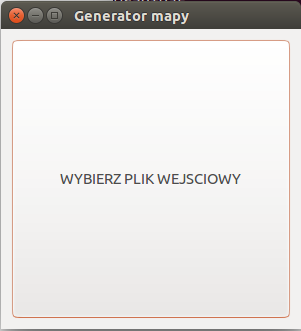
\includegraphics[ scale = 0.5 ] {wybor}
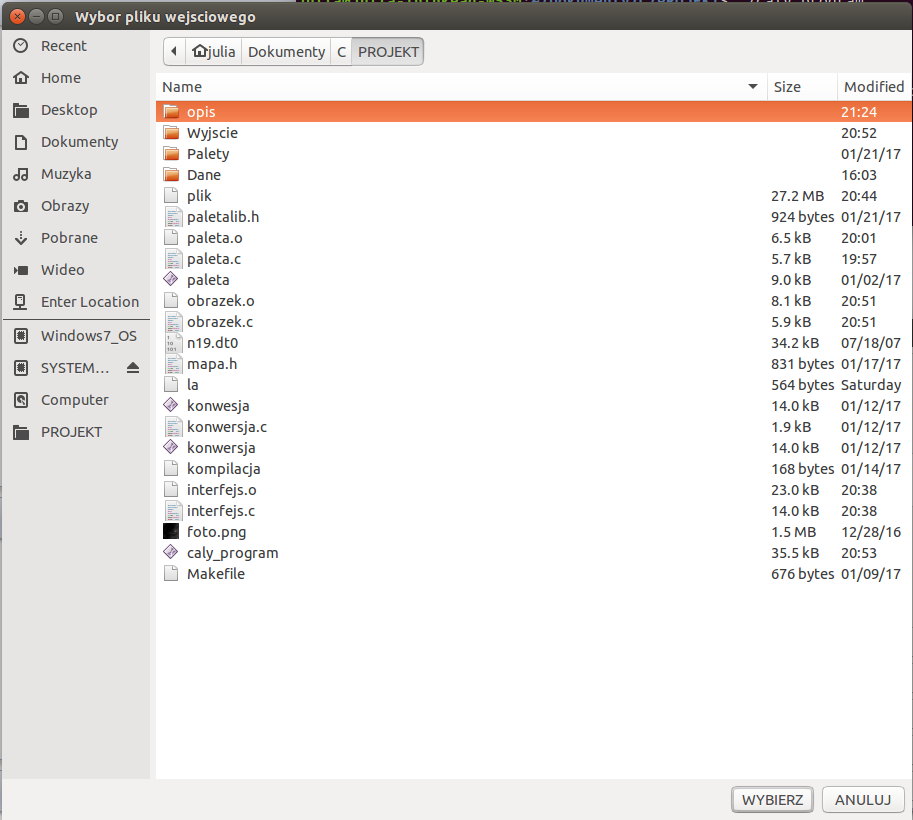
\includegraphics[scale = 0.40]{oknowyboru}

Po wybraniu pliku pojawią się dodatkowe elementy:
\begin{enumerate}
\item{Przycisk WCZYTAJ PALETĘ}\\
Przycisk umożliwia wybranie  w osobnym okienku pliku z paletą, którą następnie będzie można zaaplikować do mapy wysokości, lub zmodyfikować.
 
\item{Przycisk ZAPISZ PALETĘ}\\
Przycisk umożliwia zapisanie stanu aktualnie modyfikowanej palety do nowego lub istniejącego pliku. Plik docelowy wybiera się w osobnym okienku.

\item{Przycisk ZASTOSUJ PALETE DOMYŚLNĄ}\\
Po naciśnięciu przycisku generuje się domyślną paletę, z kolorami typowymi dla mapy hipsometrycznej. Poziomice są dostosowane do pliku z mapą w taki sposób, aby uwzględnić zakres wysokości.  

\item{Przycisk ODŚWIEŻ PODGLĄD}\\
Przycisk aktualizuje podgląd o wprowadzone zmiany w palecie. Przy plikach o rozmiarze powyżej 15 MB podgląd może się nie ładować natychmiastowo

\item{Przycisk ZAPISZ MAPĘ}\\
Przycisk umożliwia zapisanie stanu aktualnie modyfikowanej mapy do nowego lub istniejącego pliku. Plik docelowy wybiera się w osobnym okienku. Mapa zapisuje się w formacie PNG.

\item{Przycisk NOWA POZIOMICA}\\
Po naciśnieciu przycisku pojawi sie nowa poziomica do zmodyfikowania.

\item{Przycisk WYCZYŚĆ POZIOMICE}\\
Przycisk usuwa wszystkie (!) poziomice z aktualnie modyfikowanej palety.
 
\item{Pole podglądu}\\
 Pojawia się rówinież czarne pole z podglądem oraz, po jego prawej stronie, przyciski do powiększania i pomniejszania podglądu. Jeżeli wielkość podglądu przekroczy rozmiary pola można poruszać się po podglądzie przy pomocy suwaków z prawej strony i od dołu pola podglądu.
 
\item{Poziomice}\\
 Pojawiają się po wczytaniu palety, lub po dodaniu poziomicy. Na każdej znajdują się :
 	\begin{enumerate}
 	\item{}
 	Pole tekstowe  do wpisania warości liczbowej poziomicy w metrach. Wartość poziomicy się zmienia po wpisaniu - nie trzeba wciskać dodatkowo Enter. Do momentu wpisania wartości liczbowej poziomica nie jest aktywna. Wpisanie czegoś innego niż liczba powoduje przypisanie poziomicy wartości domyślnej 0. Wartość poziomicy stanowi górne ograniczenie wartości punktów pokolorowany na dany kolor.
 	
 	Uwaga! W niektórych plikach wartości 1 w pliku mapy wysokości jest przypisana jest inna wartość niż 1 metr. Wtedy ciężar przeliczenia wartości poziomic spoczywa na użytkowniku.
 	\item{}
 	Przycisk zaznaczony kolorem (domyślnie seledynowym) służący do ustawiania poziomicy koloru . Po naciśnięciu go wyskakuje okienku wyboru barwy, w którym można wybrać z pośród istniejących kolorów lub zmieszać własny. Po wybraniu koloru przycisk zmienia kolor na wybrany.
 	\item{}
 	Przycisk usuń trwale usuwa poziomicę z palety
 	\end{enumerate}
  \end{enumerate}
 
  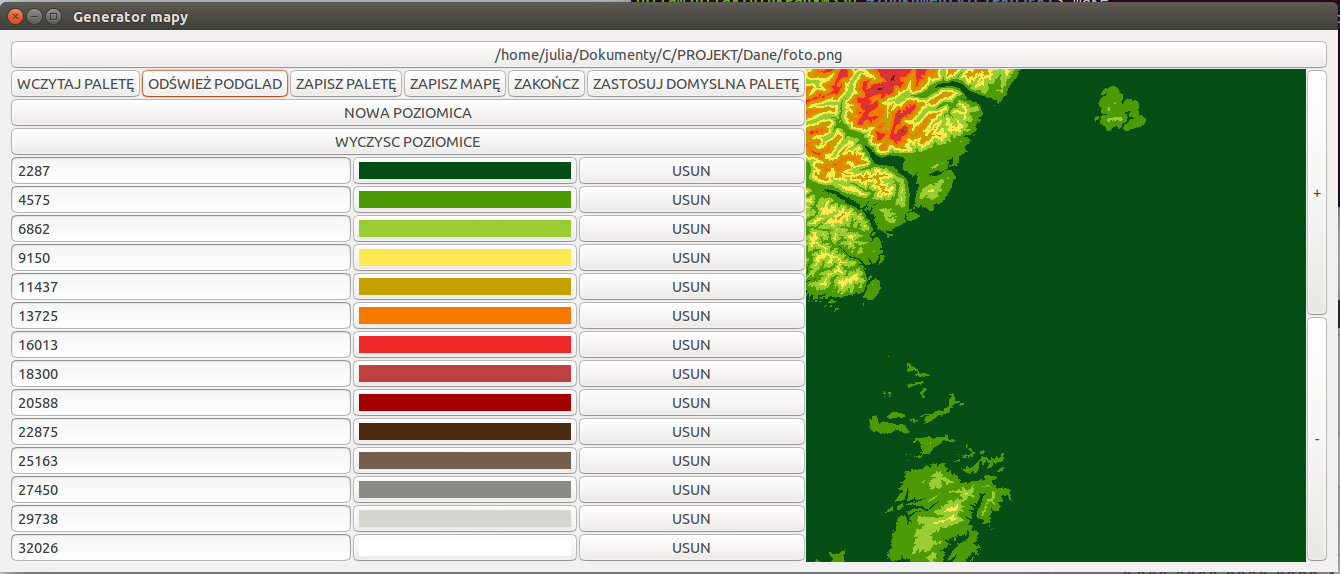
\includegraphics[scale=0.4]{zmapa}\\
  Wszelkie komunikaty o błędach wypisywane są na standardowe wyjście
 \section{Plik paleta.c}
 Plik korzysta z fukcji bibliotek zewnętrznych GTK oraz stdio oraz stdlib oraz funkcji ustaw\textunderscore poziomice z modułu interfejs
 
 Biblioteka opiera się na dwóch stukturach:
  \begin{enumerate}
  \item{poziom}
  \begin{lstlisting}
  
  struct poziom{
    int wysokosc;
    GdkRGBA kolor;
    struct poziom* nastepny;
    struct poziom* poprzedni;
   };
  
  \end{lstlisting}
  Struktura reprezentuje element listy poziomic i zawiera całkowitoliczbową wysokość, kolor w postaci struktury GdkRGBA oraz wskaźniki na poprzedni oraz następny element listy.
  
   Korzystam z następujących funkcji do tej struktury:
   \begin{enumerate}   
   
  \item{poziom* nowy\textunderscore poziom( paleta *pal,  int w, GdkRGBA kol)} --- funkcja alokująca pamięc pod strukturę poziom i zwracająca wskaźnik na nią. Ustawia wartość wyskokościi na w i wartość kolor na kol oraz wstawiająca ją w odpowiednie miejsce w palecie pal ( kolejność w strukturze jest zgodna z wysokościami).
  
  \item{void usun\textunderscore poziom(poziom *p, paleta *pal)} --- funkcja zwalniająca pamięć struktury poziom oraz usuwająca go ze struktury pal.
  
  \item{poziom* przenies(poziom* nowy, paleta* pal);} - funkcja aktualizująca położenie danego poziomu w palecie zgodnie z wpisaną wysokością.
  
  
  \end{enumerate}
  \item{paleta}
  \begin{lstlisting}
  typedef struct {
    poziom* p; 
    poziom* k;
  } paleta;  
  \end{lstlisting}  
  Struktura reprezentuje listę poziomic i trzyma jej pierwszy i ostatni element.
  
  Korzystam z następujących funkcji do tej struktury:
  \begin{enumerate}
  \item{paleta* nowa\_ paleta()} --- funkcja alokująca pamięc pod strukturę paleta i zwracająca wskaźnik na nią.
  
  \item{void usun\_ palete(paleta *pal)} --- funkcja zwalniająca pamięc struktury paleta.
   
  \item{void wyczysc\_ palete(paleta *pal)} --- funkcja niszcząca wszystkie poziomice w strukturze paleta.
  
  \item{paleta* wczytaj\_ palete(char* nazwa\_ pliku, GtkWidget* pudelko, paleta* p) } --- funkcja wczytuje paletę z pliku o ścieżce zapisanej w nazwa\_ pliku do palety p (jeśli p to NULL to tworzy nową paletę) oraz dodaje reprezentację poziomic do kontenera gtk pudelko.
  
  \item{void zapisz\_ palete( paleta* p, char* nazwa\_ pliku)} --- funkcja zapisująca paletę p do pliku o ścieżce zapisanej w nazwa\_ pliku.
  
  \item{paleta* paleta\_ domyslna(int min, int max, GtkWidget *pudelko, paleta* pal)} --- funkcja tworząca domyślną paletę kolorów w palecie pal dla danej wartości minialnej i maksymalnej występującej na mapie. Funkcja tworzy również reprezentacje graficzną palety w kontenerze GTK pudelko.
  
  \end{enumerate}
  \end{enumerate}
  Dodatkowo została zaimplementowana fukcja pomocnicza void zniszcz(GtkWidget* widget, gpointer dane) służąca do niszczenia widgetu podanego jako pierwszy argument
  
  \section{Plik obrazek.c}
  W tym pliku znajdują się funkcje związane z operacjami na mapie wysokości.
  
 
	\textbf{Struktura mapa}
  	\begin{lstlisting}
  typedef struct{
    int h, w, maxval, minval;
    int ** obraz;
        
  }mapa;
   \end{lstlisting}  
   
  \textbf{Funkcje}
  \begin{enumerate}
  
  \item{mapa* stworz\_ nowa\_ mape(int h, int w)}\\
  Funkcja alokuje pamięc na strukturę mapa o wysokosci h i szerokości h.
  
  \item{void zniszcz\_ mape(mapa *m)}\\
  Funkcja zwalnia pamięć struktury pod wskaźnikiem m. Zwalnia też wszystkie zawarte w niej wskaźniki.
  
  \item{mapa* wczytaj\_ mape\_ z\_ formatu(char* nazwa)}\\
  \textit{kod zaczerpniety z http://www.gdal.org/gdal\textunderscore tutorial.html}\\
  Funkcja wczytuje plik o ścieżce zapisanej w nazwa przy pomocy biblioteki gdal. Wczytuje jedynie pierwszą warstwę barwną zgodnie ze standardową specyfikacją pilku mapy wysokości. Zapisuje dane w nowo utworzonej strukturze typu mapa. Dane są wczytywane jako 16-bitowy integer ze znakiem, dane wykraczające poza zakres zostaną zaminione na maksymalną wartość 16-bitowego inta. Korzystam z funkcji biblioteki GDAL aby obliczyć minimalną i maksymalną wysokość na mapie. 
  
  \item{void zapisz\_ mape\_ do\_ pliku(mapa* m, paleta * pal,const char* nazwa)}\\
  Funkcja zapisuje mapę kolorową będącą mapą wysokości m z zaaplikowaną paletą pal do pliku o ścieżce zapisanej w nazwa/
  
   \item{GdkPixbuf* zamien\_ na\_ kolorki(paleta* pal, mapa* m)}\\
   Funkcja zamieniająca mapę wysokości na nową strukturę GdkPixbuf wraz z nadaniem pixelom kolorów zgonie z paletą. 
   
   \item{void zmien\textunderscore pixel( GdkPixbuf* imageptr, int x, int y, GdkRGBA* kol)}\\
   \textit{ kod pochodzi z tej strony http://stackoverflow.com/questions/16785886/get-pixel-value-on-gdkpixbuf-set-pixel-value-with-gdkcairo}\\
	Funkcja ustawiająca kolor pixela o współrzędnych x, y w GdkPixbuf na kol.
	
	\item{GdkRGBA* znajdz\textunderscore kolor(int wysokosc, paleta* pal)}\\
	Funkcja znajdująca kolor odpowiadajacy wysokości dla danej palety.
	
	\item{short get\textunderscore green(GdkRGBA* kolor)}\\
	Funkcja zamienia zmiennoprzecinkową składową zieloną na wartość 8-bitowego inta tak jak w strukturze GdkPixbuf.
	
	\item{short get\textunderscore red(GdkRGBA* kolor)}\\
	Funkcja zamienia zmiennoprzecinkową składową czerwoną na wartość 8-bitowego inta tak jak w strukturze GdkPixbuf.
	
	\item{short get\textunderscore blue(GdkRGBA* kolor)}\\
	Funkcja zamienia zmiennoprzecinkową składową niebieską na wartość 8-bitowego inta tak jak w strukturze GdkPixbuf.

  \end{enumerate}
\section{Plik interfejs.c}

Moduł główny programu. Implementuje interfejs oraz wszystkie funkcje programu.

\begin{enumerate}
\item{Operacje na plikach}\\
Do wczytywania i zapisu plików wykorzystany został widget GtkFileChooserDialog. Kod obsługi tego widgetu został zaczerpnięty ze strony \textit{https://developer.gnome.org/gtk3/stable/GtkFileChooserDialog.html}.
 
\item{Wybór koloru}\\
Do wyboru koloru dla poziomicy wykorzystano widget GtkColorChooserButton.

\item{Wprowadzanie wysokości}\\
Do wprowadzania wysokości służy widget GtkEntry. Wpowadzony tam tekst zostanie przekształcony przez funkcję atoi na liczbę. \\
Dla poziomicy stworzonej w oknie początkowo ustawiony jest tekst startowy funkcją gtk\_ set\_ placeholder\_ text.\\
Dla wczytanych poziomic tekst jest ustawiany przy pomocy gtk\_ set\_ text na wartość poziomicy.\\
Wartość poziomicy jest aktualizowana po każdej zmianie w tym polu.
 
\item{Podgląd}\\
Podgląd jest tworzony poprzez konwersję do widgetu GdkPixbuf a następnie wyświetlany jako GtkImage.

Do poruszania się po podglądzie został użyty widget GtkScrolledWindow.

Powiększenie (analogicznie pomniejszenie) podglądu odbywa się przez pomnożenie przez 2 globalnej zmiennej typu double enlargement, a następnie przeskalowaniu widgetu GdkPixbuf, zawierającego obraz w początkowej rozdzielczości, o tą zmienną. Wykorzystana została funkcja gdk\_ pixbuf\_ scale() z opcją GDK\_ INTERP\_ BILINEAR.

Po odświeżeniu obraz się skaluje do szerokości 500 pixeli i proporcjonalnej wysokości.

Podgląd jest ładowany 5 sekund po ostatniej modyfikacji w palecie, lub od razu po zmianie pliku wejściowego, wczytaniu nowej palety lub zastosowaniu palety domyślnej. Przy plikach o rozmiarze powyżej 15mb podgląd może się nie ładować natychmiastowo.

\item{Kolejność poziomic}\\
 5 sekund po wprowadzeniu ostatniej zmiany w palecie poziomice sortują się automatycznie rosnąco względem wysokości.
\end{enumerate}

\section{Źródła map}
\href{www.cc.gatech.edu/projects/large_models/ps.html}{Mapy zachodniego wybrzeża Stanów Zjednoczonych w formacie PNG}

\href{http://www.viewfinderpanoramas.org/Coverage\%20map\%20viewfinderpanoramas_org3.htm}{Wyszukiwarka map w formacie HGT }

\href{http://srtm.csi.cgiar.org/SELECTION/inputCoord.asp}{Wyszukiwarka map w formacie TIFF}

\href{http://data.geocomm.com/catalog/index.html}{Wyszukiwarka map w formacie DTED}

\section{Źródła używane przy pisaniu programu}

\href{https://developer.gnome.org/}{Centrum programistyczne GNOME}

\href{www.gdal.org}{Strona główna biblioteki GDAL}

\end{document}

